\section*{\fs{12}Zapytanie z podzapytaniem w Where}
\par{
\fs{12}
\subsection*{\fs{12} Imię, nazwisko i wypłatę najlepiej zarabiającego pracownika specjalizującego się w specjalizacji o ID 3.}

\listsinglespacing{
\fs{12}
\begin{lstlisting}[frame=single,language=SQL,]
SELECT imie, nazwisko, wypłata
FROM Pracownicy
WHERE id_pracownika IN 
(SELECT id_pracownika 
FROM Pracownicy_specjalizacje 
WHERE id_specjalizacji = 3)
AND wypłata = (SELECT MAX(wypłata) 
FROM Pracownicy WHERE
id_pracownika IN
(SELECT id_pracownika FROM Pracownicy_specjalizacje WHERE id_specjalizacji = 3))

\end{lstlisting}
\begin{figure}[h!]
    \centering
   \scalebox{.85}{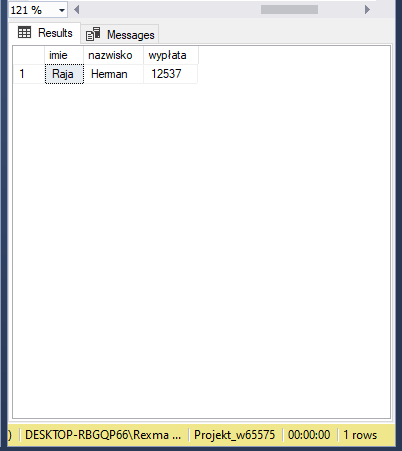
\includegraphics{Images/Zadanie3/P6/Z26a.png}}
    \caption{Wynik Zapytania}
    \label{fig:my_label}
\end{figure}
}
}
\begin{figure}[h!]
    \centering
   \scalebox{.50}{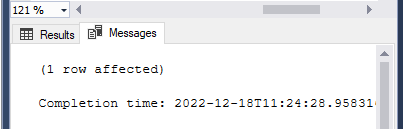
\includegraphics{Images/Zadanie3/P6/Z26b.png}}
    \caption{Wynik Zapytania}
    \label{fig:my_label}
\end{figure}
\newpage
\clearpage
\subsection*{\fs{12} Daty badań przeprowadzonych przez lekarzy z starzem pracy  większym niż 10 lat, posortowane według daty}


\listsinglespacing{
\fs{12}
\begin{lstlisting}[frame=single,language=SQL,]
SELECT convert(varchar, data, 107) AS data
FROM Badania 
WHERE lekarz IN (SELECT P.id_pracownika FROM Pracownicy AS P
WHERE DATEDIFF(year,P.data_zatrudnienia,GETDATE())>10)
order by year(data)
\end{lstlisting}
\begin{figure}[h!]
    \centering
   \scalebox{.85}{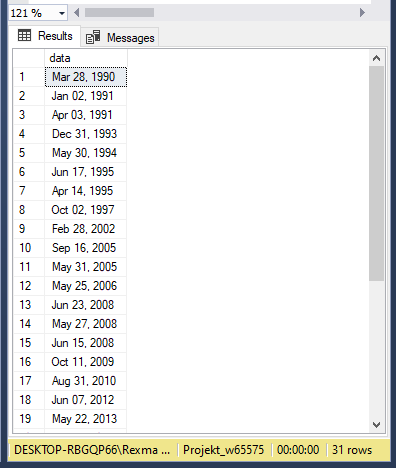
\includegraphics{Images/Zadanie3/P6/Z27a.png}}
    \caption{Wynik Zapytania}
    \label{fig:my_label}
\end{figure}
}
\begin{figure}[h!]
    \centering
   \scalebox{.50}{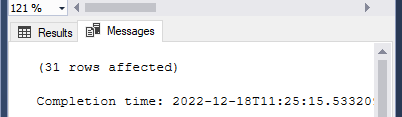
\includegraphics{Images/Zadanie3/P6/Z27b.png}}
    \caption{Wynik Zapytania}
    \label{fig:my_label}
\end{figure}

\newpage
\clearpage
\subsection*{\fs{12} Pacjenci  z Bydgoszczy}


\listsinglespacing{
\fs{12}
\begin{lstlisting}[frame=single,language=SQL,]
Select * 
from Pacjent
Where id_adres IN (Select id_adres from Adresy where miasto='Bydgoszcz')
\end{lstlisting}
\begin{figure}[h!]
    \centering
   \scalebox{.85}{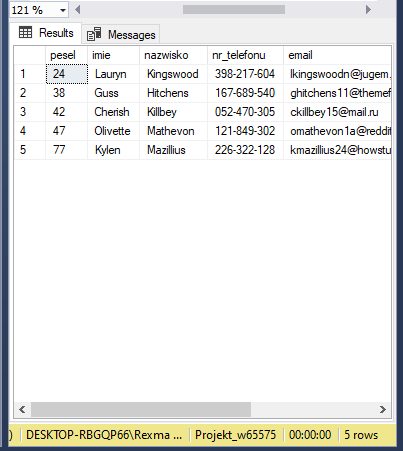
\includegraphics{Images/Zadanie3/P6/Z28a.png}}
    \caption{Wynik Zapytania}
    \label{fig:my_label}
\end{figure}
}
\begin{figure}[h!]
    \centering
   \scalebox{.60}{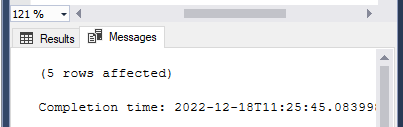
\includegraphics{Images/Zadanie3/P6/Z28b.png}}
    \caption{Wynik Zapytania}
    \label{fig:my_label}
\end{figure}


\newpage